% Options for packages loaded elsewhere
\PassOptionsToPackage{unicode}{hyperref}
\PassOptionsToPackage{hyphens}{url}
\PassOptionsToPackage{dvipsnames,svgnames*,x11names*}{xcolor}
%
\documentclass[
  ignorenonframetext,
]{beamer}
\usepackage{pgfpages}
\setbeamertemplate{caption}[numbered]
\setbeamertemplate{caption label separator}{: }
\setbeamercolor{caption name}{fg=normal text.fg}
\beamertemplatenavigationsymbolsempty
% Prevent slide breaks in the middle of a paragraph
\widowpenalties 1 10000
\raggedbottom
\setbeamertemplate{part page}{
  \centering
  \begin{beamercolorbox}[sep=16pt,center]{part title}
    \usebeamerfont{part title}\insertpart\par
  \end{beamercolorbox}
}
\setbeamertemplate{section page}{
  \centering
  \begin{beamercolorbox}[sep=12pt,center]{part title}
    \usebeamerfont{section title}\insertsection\par
  \end{beamercolorbox}
}
\setbeamertemplate{subsection page}{
  \centering
  \begin{beamercolorbox}[sep=8pt,center]{part title}
    \usebeamerfont{subsection title}\insertsubsection\par
  \end{beamercolorbox}
}
\AtBeginPart{
  \frame{\partpage}
}
\AtBeginSection{
  \ifbibliography
  \else
    \frame{\sectionpage}
  \fi
}
\AtBeginSubsection{
  \frame{\subsectionpage}
}
\usepackage{amsmath,amssymb}
\usepackage{lmodern}
\usepackage{ifxetex,ifluatex}
\ifnum 0\ifxetex 1\fi\ifluatex 1\fi=0 % if pdftex
  \usepackage[T1]{fontenc}
  \usepackage[utf8]{inputenc}
  \usepackage{textcomp} % provide euro and other symbols
\else % if luatex or xetex
  \usepackage{unicode-math}
  \defaultfontfeatures{Scale=MatchLowercase}
  \defaultfontfeatures[\rmfamily]{Ligatures=TeX,Scale=1}
\fi
% Use upquote if available, for straight quotes in verbatim environments
\IfFileExists{upquote.sty}{\usepackage{upquote}}{}
\IfFileExists{microtype.sty}{% use microtype if available
  \usepackage[]{microtype}
  \UseMicrotypeSet[protrusion]{basicmath} % disable protrusion for tt fonts
}{}
\makeatletter
\@ifundefined{KOMAClassName}{% if non-KOMA class
  \IfFileExists{parskip.sty}{%
    \usepackage{parskip}
  }{% else
    \setlength{\parindent}{0pt}
    \setlength{\parskip}{6pt plus 2pt minus 1pt}}
}{% if KOMA class
  \KOMAoptions{parskip=half}}
\makeatother
\usepackage{xcolor}
\IfFileExists{xurl.sty}{\usepackage{xurl}}{} % add URL line breaks if available
\IfFileExists{bookmark.sty}{\usepackage{bookmark}}{\usepackage{hyperref}}
\hypersetup{
  pdftitle={Chapter 7},
  colorlinks=true,
  linkcolor=Maroon,
  filecolor=Maroon,
  citecolor=Blue,
  urlcolor=blue,
  pdfcreator={LaTeX via pandoc}}
\urlstyle{same} % disable monospaced font for URLs
\newif\ifbibliography
\usepackage{graphicx}
\makeatletter
\def\maxwidth{\ifdim\Gin@nat@width>\linewidth\linewidth\else\Gin@nat@width\fi}
\def\maxheight{\ifdim\Gin@nat@height>\textheight\textheight\else\Gin@nat@height\fi}
\makeatother
% Scale images if necessary, so that they will not overflow the page
% margins by default, and it is still possible to overwrite the defaults
% using explicit options in \includegraphics[width, height, ...]{}
\setkeys{Gin}{width=\maxwidth,height=\maxheight,keepaspectratio}
% Set default figure placement to htbp
\makeatletter
\def\fps@figure{htbp}
\makeatother
\setlength{\emergencystretch}{3em} % prevent overfull lines
\providecommand{\tightlist}{%
  \setlength{\itemsep}{0pt}\setlength{\parskip}{0pt}}
\setcounter{secnumdepth}{-\maxdimen} % remove section numbering
\usepackage{multirow} \usepackage{graphicx} \graphicspath{{images/}} \usepackage{subfigure} \usepackage{multicol} \usepackage[utf8]{inputenc} \usepackage[english]{babel} \usepackage{bm} \usepackage{amsmath} \usepackage{tikz} \usepackage{mathtools} \usepackage{textcomp} \usepackage{fdsymbol} \usepackage{siunitx} \usepackage{xcolor,pifont} \usepackage{hyperref} \usepackage{mathtools}
\ifluatex
  \usepackage{selnolig}  % disable illegal ligatures
\fi

\title{Chapter 7}
\subtitle{Inference for numerical data\footnote<.->{These notes use
  content from OpenIntro Statistics Slides by Mine Cetinkaya-Rundel.}}
\author{Department of Mathematics \& Statistics\\
North Carolina A\&T State University}
\date{}

\begin{document}
\frame{\titlepage}

\hypertarget{comparing-mean-with-anova}{%
\section{Comparing mean with ANOVA}\label{comparing-mean-with-anova}}

\begin{frame}{}
\protect\hypertarget{section}{}
\centering

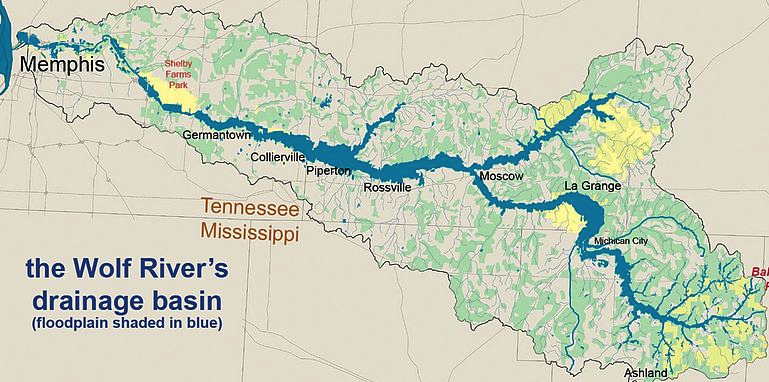
\includegraphics[width=\textwidth,height=0.25\textheight]{images/wolf.png}

\begin{itemize}
\tightlist
\item
  The Wolf River in Tennessee flows past an abandoned site once used by
  the pesticide industry for dumping wastes, including chlordane
  (pesticide), aldrin, and dieldrin (both insecticides).
\end{itemize}

\pause

\begin{itemize}
\tightlist
\item
  These highly toxic organic compounds can cause various cancers and
  birth defects.
\end{itemize}

\pause

\begin{itemize}
\tightlist
\item
  The standard methods to test whether these substances are present in a
  river is to take samples at six-tenth depth.
\end{itemize}

\pause

\begin{itemize}
\tightlist
\item
  But since these compounds are denser than water and their molecules
  tend to stick to particles of sediment, they are more likely to be
  found in higher concentrations near the bottom than near mid depth.
\end{itemize}
\end{frame}

\begin{frame}{Data}
\protect\hypertarget{data}{}
Aldrin concentration (nanograms per liter) at three levels of depth.

\begin{center}
\begin{tabular}{r | c | c}
\hline
    & aldrin                    & depth \\ 
\hline
1   & \textcolor{gray}{3.80}    & \textcolor{gray}{bottom}  \\ 
2   & \textcolor{gray}{4.80}    & \textcolor{gray}{bottom}  \\ 
... &                       & \\
10  & \textcolor{gray}{8.80}    & \textcolor{gray}{bottom} \\
11  & \textcolor{blue}{3.20}        & \textcolor{blue}{middepth}  \\
12  & \textcolor{blue}{3.80}        & \textcolor{blue}{middepth} \\
... &                       & \\
20  & \textcolor{blue}{6.60}        & \textcolor{blue}{middepth} \\
21  & \textcolor{green}{3.10}       & \textcolor{green}{surface} \\
22  & \textcolor{green}{3.60}       & \textcolor{green}{surface} \\
... &                       & \\
30  & \textcolor{green}{5.20}       & \textcolor{green}{surface} \\  
\hline
\end{tabular}
\end{center}
\end{frame}

\begin{frame}{Exploratory analysis}
\protect\hypertarget{exploratory-analysis}{}
Aldrin concentration (nanograms per liter) at three levels of depth.

\begin{center}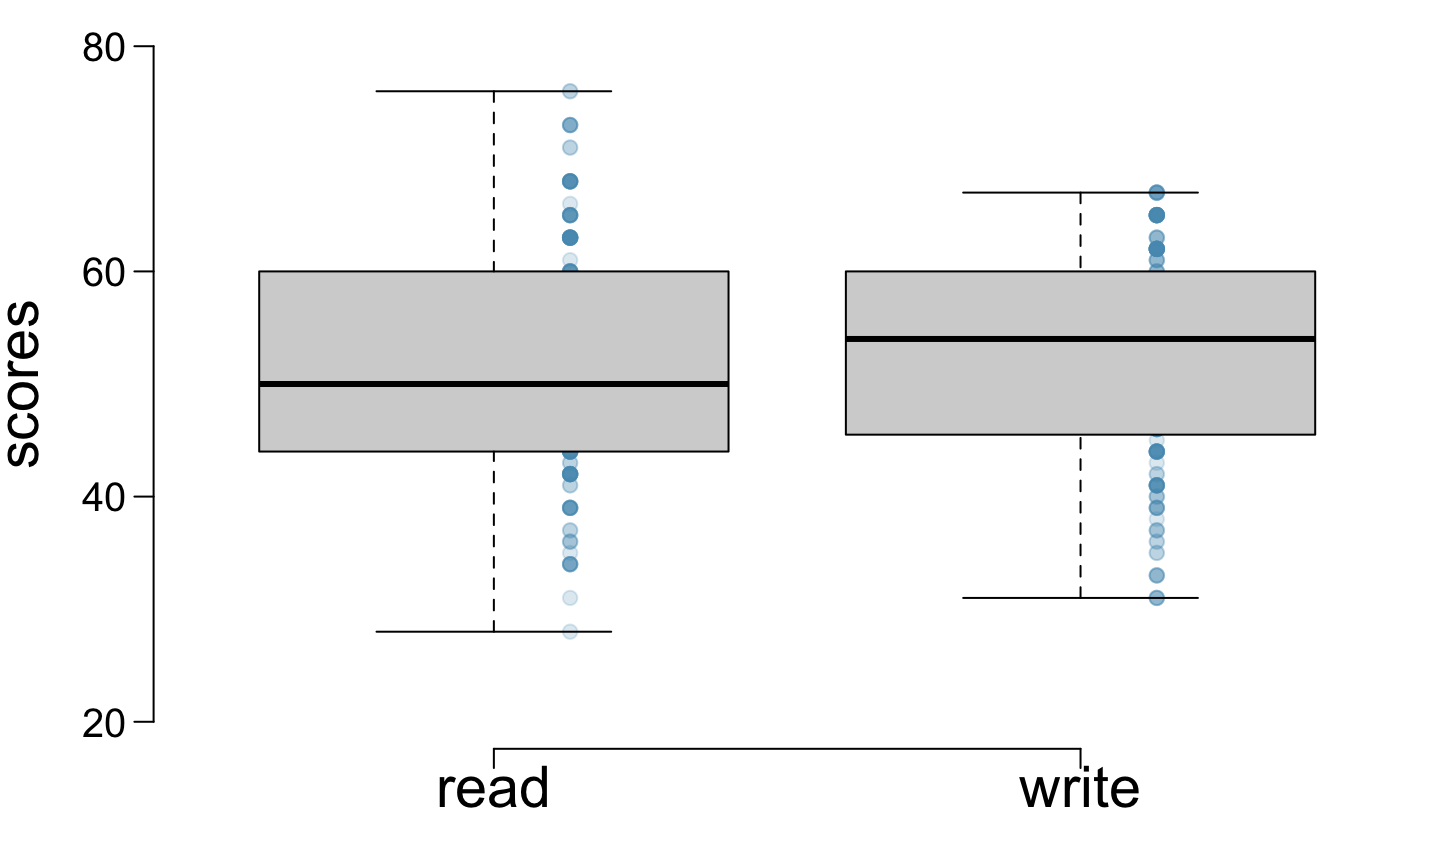
\includegraphics{Section7.5-ComparingMeanWithANOVA_files/figure-beamer/unnamed-chunk-2-1} \end{center}

\begin{center}
\begin{tabular}{l | c c c}
        & n & mean  & sd        \\
\hline
bottom  & 10    & 6.04  & 1.58 \\
middepth& 10    & 5.05  & 1.10 \\
surface & 10    & 4.20  & 0.66 \\
\hline
overall & 30    & 5.1   0   & 1.37
\end{tabular}
\end{center}
\end{frame}

\begin{frame}{Research question}
\protect\hypertarget{research-question}{}
\alert{Is there a difference between the mean aldrin concetrations among the three levels?}

\pause

\begin{itemize}
\tightlist
\item
  To compare means of 2 groups we use a Z or a T statistic.
\end{itemize}

\pause

\begin{itemize}
\tightlist
\item
  To compare means of 3+ groups we use a new test called \textbf{ANOVA}
  and a new statistic called \textbf{F}.
\end{itemize}
\end{frame}

\begin{frame}{ANOVA}
\protect\hypertarget{anova}{}
ANOVA is used to assess whether the mean of the outcome variable is
different for different levels of a categorical variable.

\begin{itemize}
\item[$H_0:$] The mean outcome is the same across all categories,\[\mu_1 = \mu_2 = \cdots = \mu_k, \]
where $\mu_i$ represents the mean of the outcome for observations in category $i$.
\item[]
\item[$H_A:$] At least one mean is different than others.
\end{itemize}
\end{frame}

\begin{frame}{Conditions}
\protect\hypertarget{conditions}{}
\begin{enumerate}

\item The observations should be independent within and between groups

\begin{itemize}
\item If the data are a simple random sample from less than 10\% of the population, this condition is satisfied.
\item Carefully consider whether the data may be independent (e.g. no pairing). 
\item Always important, but sometimes difficult to check.
\end{itemize}

\pause

\item The observations within each group should be nearly normal.

\begin{itemize}
\item Especially important when the sample sizes are small.
\end{itemize}

\alert{How do we check for normality?}

\pause

\item The variability across the groups should be about equal.

\begin{itemize}
\item Especially important when the sample sizes differ between groups.
\end{itemize}

\alert{How can we check this condition?}

\end{enumerate}
\end{frame}

\begin{frame}{\(z/t\) test vs.~ANOVA - Purpose}
\protect\hypertarget{zt-test-vs.-anova---purpose}{}
\begin{columns}

\begin{column}{0.45\textwidth}
\centering{$\mathbf{z/t}$ \textbf{test}}

\raggedright Compare means from \textbf{two} groups to see whether they are so far apart that the observed difference cannot reasonably be attributed to sampling variability.


\centering{$H_0: \mu_1=\mu_2$}
\end{column}

\begin{column}{0.45\textwidth}
\centering{\textbf{ANOVA}}

\raggedright Compare the means from \textbf{two or more} groups to see whether they are so far apart that the observed difference cannot all reasonably be attributed to sampling variability.


\centering{$H_0: \mu_1=\mu_2= \cdots = \mu_k$}
\end{column}

\end{columns}
\end{frame}

\begin{frame}{\(z/t\) test vs.~ANOVA - Method}
\protect\hypertarget{zt-test-vs.-anova---method}{}
\begin{columns}

\begin{column}{0.45\textwidth}
\centering{$\mathbf{z/t}$ \textbf{test}}

\raggedright Compare a test statistic (a ratio).


\centering{$z/t = \frac{(\bar{x}_1 - \bar{x}_2) - (\mu_1-\mu_2)}{SE(\bar{x}_1-\bar{x}_2)}$}
\end{column}

\begin{column}{0.45\textwidth}
\centering{\textbf{ANOVA}}

\raggedright Compare a test statistic (a ratio).


\centering{$F = \frac{\text{variability bet. groups}}{\text{variability w/in groups}}$}
\end{column}

\end{columns}

\pause

\begin{itemize}
\item
  Large test statistics lead to small p-values.
\item
  If the p-value is small enough \(H_0\) is rejected, we conclude that
  the population means are not equal.
\end{itemize}
\end{frame}

\begin{frame}{\(z/t\) test vs.~ANOVA}
\protect\hypertarget{zt-test-vs.-anova}{}
\begin{itemize}
\tightlist
\item
  With only two groups t-test and ANOVA are equivalent, but only if we
  use a pooled standard variance in the denominator of the test
  statistic.
\end{itemize}

\pause

\begin{itemize}
\tightlist
\item
  With more than two groups, ANOVA compares the sample means to an
  overall \textbf{grand mean}.
\end{itemize}
\end{frame}

\begin{frame}{Hypotheses}
\protect\hypertarget{hypotheses}{}
\alert{What are the correct hypotheses for testing for a difference between the mean aldrin concentrations among the three levels?}

\begin{enumerate}[(a)]
\item $H_0: \mu_B = \mu_M = \mu_S$ \\
$H_A: \mu_B \ne \mu_M \ne \mu_S$ \\
\item $H_0: \mu_B \ne \mu_ M \ne \mu_S$ \\
$H_A: \mu_B = \mu_M = \mu_S$ \\
\item $H_0: \mu_B = \mu_M = \mu_S$ \\
$H_A:$ At least one mean is different.
\item $H_0: \mu_B = \mu_M = \mu_S = 0$ \\
$H_A:$ At least one mean is different.
\item $H_0: \mu_B = \mu_M = \mu_S$ \\
$H_A: \mu_B > \mu_M > \mu_S$ \\
\end{enumerate}
\end{frame}

\begin{frame}{Hypotheses}
\protect\hypertarget{hypotheses-1}{}
\alert{What are the correct hypotheses for testing for a difference between the mean aldrin concentrations among the three levels?}

\begin{enumerate}[(a)]
\item $H_0: \mu_B = \mu_M = \mu_S$ \\
$H_A: \mu_B \ne \mu_M \ne \mu_S$ \\
\item $H_0: \mu_B \ne \mu_ M \ne \mu_S$ \\
$H_A: \mu_B = \mu_M = \mu_S$ \\
\item \alert{$H_0: \mu_B = \mu_M = \mu_S$} \\
\alert{$H_A:$ At least one mean is different.}
\item $H_0: \mu_B = \mu_M = \mu_S = 0$ \\
$H_A:$ At least one mean is different.
\item $H_0: \mu_B = \mu_M = \mu_S$ \\
$H_A: \mu_B > \mu_M > \mu_S$ \\
\end{enumerate}
\end{frame}

\begin{frame}{Test statistic}
\protect\hypertarget{test-statistic}{}
\alert{Does there appear to be a lot of variability within groups? How about between groups?}

\centering{$F = \frac{\text{variability bet. groups}}{\text{variability w/in groups}}$}

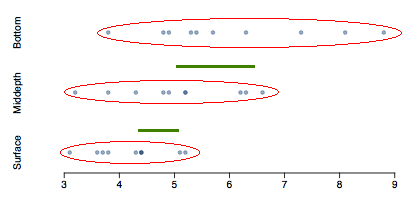
\includegraphics[width=\textwidth,height=0.4\textheight]{images/dotplot_var.png}
\end{frame}

\begin{frame}{\(F\) distribution and p-value}
\protect\hypertarget{f-distribution-and-p-value}{}
\centering{$F = \frac{\text{variability bet. groups}}{\text{variability w/in groups}}$}

\begin{center}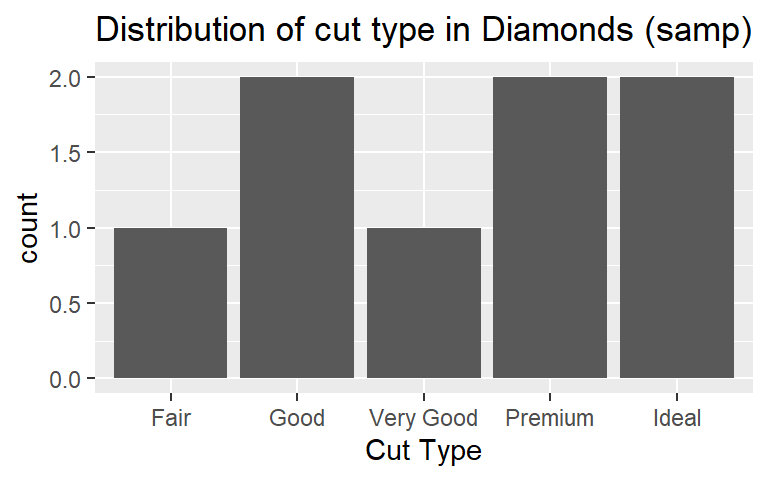
\includegraphics{Section7.5-ComparingMeanWithANOVA_files/figure-beamer/unnamed-chunk-3-1} \end{center}

\begin{itemize}
\item
  In order to be able to reject \(H_0\), we need a small p-value, which
  requires a large F statistic.
\item
  In order to obtain a large F statistic, variability between sample
  means needs to be greater than variability within sample means.
\end{itemize}
\end{frame}

\begin{frame}{Degrees of freedom associated with ANOVA}
\protect\hypertarget{degrees-of-freedom-associated-with-anova}{}
\begin{center}
\begin{tabular}{llrrrrr}
\hline
            &           & Df    & Sum Sq    & Mean Sq   & F value   & Pr($>$F) \\ 
\hline
(\alert{G}roup)     & depth         & 2     & 16.96     & 8.48      & 6.13  & 0.0063 \\ 
(\alert{E}rror)     & Residuals     & 27    & 37.33     & 1.38      &       &  \\ 
\hline
            & \alert{T}otal & 29    & 54.29 \\
\end{tabular}
\end{center}

\begin{itemize}
\item groups: $df_G = k - 1$, where $k$ is the number of groups
\item total: $df_T = n - 1$, where $n$ is the total sample size
\item error: $df_E = df_T - df_G$
\end{itemize}

\pause

\begin{itemize}

\item $df_G = k - 1 = 3 - 1 = 2$ \\ 

\pause

\item $df_T = n - 1 = 30 - 1 = 29$

\pause

\item $df_E = 29 - 2 = 27$ \\

\end{itemize}
\end{frame}

\begin{frame}{Sum of squares between groups, SSG}
\protect\hypertarget{sum-of-squares-between-groups-ssg}{}
\footnotesize
\begin{center}
\begin{tabular}{ll rrrrr}
\hline
            &           & Df    & Sum Sq    & Mean Sq   & F value   & Pr($>$F) \\ 
\hline
(\alert{G}roup)     & depth         & 2     & \textcolor{red}{16.96}    & 8.48      & 6.13  & 0.0063 \\ 
(\alert{E}rror)     & Residuals     & 27    & 37.33     & 1.38      &       &  \\ 
\hline
            & \alert{T}otal & 29    & 54.29 \\
\end{tabular}
\end{center}

\normalsize

Measures the variability between groups \vspace{-0.25cm}
\[ SSG = \sum_{i = 1}^{k} n_i (\bar{x}_i - \bar{x})^2 \] where \(n_i\)
is each group size, \(\bar{x}_i\) is the average for each group,
\(\bar{x}\) is the overall (grand) mean.

\pause

\vspace{-0.5cm}

\begin{columns}

\begin{column}{0.4\textwidth}
\small
\begin{center}
\begin{tabular}{l | c c }
        & n & mean      \\
\hline
bottom  & 10    & 6.04   \\
middepth& 10    & 5.05   \\
surface & 10    & 4.2    \\
\hline
overall & 30    & 5.1   
\end{tabular}
\end{center}
\end{column}

\pause

\normalsize
\begin{column}{0.5\textwidth}
\begin{eqnarray*}
SSG &=& \left( 10 \times (6.04 - 5.1)^2 \right) \\
\pause
&+& \left( 10 \times (5.05 - 5.1)^2 \right) \\
\pause
&+& \left( 10 \times (4.2 - 5.1)^2 \right) \\
\pause
&=& 16.96 \\
\end{eqnarray*}
\end{column}

\end{columns}
\end{frame}

\begin{frame}{Sum of squares total, SST}
\protect\hypertarget{sum-of-squares-total-sst}{}
\begin{center}
\begin{tabular}{ll rrrrr}
\hline
            &           & Df    & Sum Sq    & Mean Sq   & F value   & Pr($>$F) \\ 
\hline
(\alert{G}roup)     & depth         & 2     & 16.96 & 8.48      & 6.13  & 0.0063 \\ 
(\alert{E}rror)     & Residuals     & 27    & 37.33     & 1.38      &       &  \\ 
\hline
            & \alert{T}otal & 29    & \textcolor{red}{54.29} \\
\end{tabular}
\end{center}

Measures the variability between groups \vspace{-0.25cm}
\[ SST = \sum_{i = 1}^{n} (x_i - \bar{x})^2 \] where \(x_i\) represent
each observation in the dataset.

\pause

\vspace{-0.75cm}

\begin{eqnarray*}
SST &=& (3.8 - 5.1)^2 + (4.8 - 5.1)^2 + (4.9 - 5.1)^2 + \cdots + (5.2 - 5.1)^2 \\
\pause
&=& (-1.3)^2 + (-0.3)^2 + (-0.2)^2 + \cdots + (0.1)^2 \\
\pause
&=& 1.69 + 0.09 + 0.04 + \cdots + 0.01 \\
\pause
&=& 54.29
\end{eqnarray*}
\end{frame}

\begin{frame}{Sum of squares error, SSE}
\protect\hypertarget{sum-of-squares-error-sse}{}
\begin{center}
\begin{tabular}{ll rrrrr}
\hline
            &           & Df    & Sum Sq    & Mean Sq   & F value   & Pr($>$F) \\ 
\hline
(\alert{G}roup)     & depth         & 2     & 16.96 & 8.48      & 6.13  & 0.0063 \\ 
(\alert{E}rror)     & Residuals     & 27    & \textcolor{red}{37.33}    & 1.38      &       &  \\ 
\hline
            & \alert{T}otal & 29    & 54.29 \\
\end{tabular}
\end{center}

Measures the variability within groups: \[ SSE = SST - SSG \]

\pause

\[ SSE =  54.29 - 16.96 =  37.33 \]
\end{frame}

\begin{frame}{Mean square error}
\protect\hypertarget{mean-square-error}{}
\begin{center}
\begin{tabular}{ll rrrrr}
\hline
            &           & Df    & Sum Sq    & Mean Sq   & F value   & Pr($>$F) \\ 
\hline
(\alert{G}roup)     & depth         & 2     & 16.96 & \textcolor{red}{8.48}         & 6.13  & 0.0063 \\ 
(\alert{E}rror)     & Residuals     & 27    & 37.33     & \textcolor{red}{1.38}         &       &  \\ 
\hline
            & \alert{T}otal & 29    & 54.29 \\
\end{tabular}
\end{center}

Mean square error is calculated as sum of squares divided by the degrees
of freedom.

\pause

\begin{eqnarray*}
MSG &=& 16.96 / 2 = 8.48 \\
\pause
MSE &=& 37.33 / 27 = 1.38
\end{eqnarray*}
\end{frame}

\begin{frame}{Test statistic, F value}
\protect\hypertarget{test-statistic-f-value}{}
\begin{center}
\begin{tabular}{ll rrrrr}
\hline
            &           & Df    & Sum Sq    & Mean Sq   & F value   & Pr($>$F) \\ 
\hline
(\alert{G}roup)     & depth         & 2     & 16.96 & 8.48      & \textcolor{red}{6.14}     & 0.0063 \\ 
(\alert{E}rror)     & Residuals     & 27    & 37.33     & 1.38      &       &  \\ 
\hline
            & \alert{T}otal & 29    & 54.29 \\
\end{tabular}
\end{center}

As we discussed before, the F statistic is the ratio of the between
group and within group variability. \[ F = \frac{MSG}{MSE} \]

\pause

\[ F = \frac{8.48}{1.38} = 6.14 \]
\end{frame}

\begin{frame}[fragile]{p-value}
\protect\hypertarget{p-value}{}
\begin{center}
\begin{tabular}{ll rrrrr}
\hline
            &           & Df    & Sum Sq    & Mean Sq   & F value   & Pr($>$F) \\ 
\hline
(\alert{G}roup)     & depth         & 2     & 16.96 & 8.48      & \textcolor{red}{6.14}     & 0.0063 \\ 
(\alert{E}rror)     & Residuals     & 27    & 37.33     & 1.38      &       &  \\ 
\hline
            & \alert{T}otal & 29    & 54.29 \\
\end{tabular}
\end{center}

p-value is the probability of at least as large a ratio between the
\texttt{between\ group"\ and}within group" variability, if in fact the
means of all groups are equal. It's calculated as the area under the F
curve, with degrees of freedom \(df_G\) and \(df_E\), above the observed
F statistic.

\pause

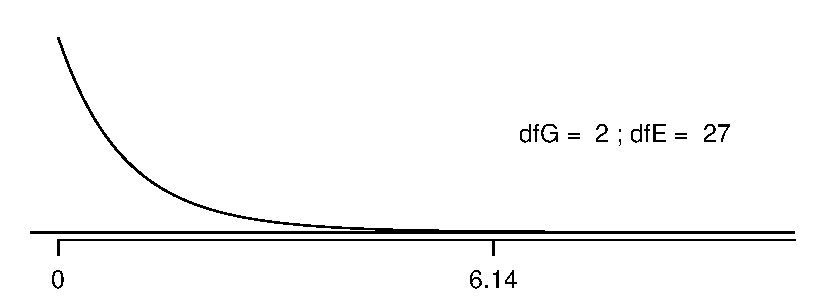
\includegraphics[width=\textwidth,height=0.45\textheight]{images/f.pdf}
\end{frame}

\begin{frame}{Conclusion - in context}
\protect\hypertarget{conclusion---in-context}{}
\alert{What is the conclusion of the hypothesis test?}

The data provide convincing evidence that the average aldrin
concentration

\begin{enumerate}
[A)]
\item
  is different for all groups.
\item
  on the surface is lower than the other levels.
\item
  is different for at least one group.
\item
  is the same for all groups.
\end{enumerate}
\end{frame}

\begin{frame}{Conclusion - in context}
\protect\hypertarget{conclusion---in-context-1}{}
\alert{What is the conclusion of the hypothesis test?}

The data provide convincing evidence that the average aldrin
concentration

\begin{enumerate}
[A)]
\item
  is different for all groups.
\item
  on the surface is lower than the other levels.
\item
  \alert{is different for at least one group.}
\item
  is the same for all groups.
\end{enumerate}
\end{frame}

\begin{frame}{Conclusion}
\protect\hypertarget{conclusion}{}
\begin{itemize}
\tightlist
\item
  If p-value is small (less than \(\alpha\)), reject \(H_0\). The data
  provide convincing evidence that at least one mean is different from
  (but we can't tell which one).
\end{itemize}

\pause

\begin{itemize}
\tightlist
\item
  If p-value is large, fail to reject \(H_0\). The data do not provide
  convincing evidence that at least one pair of means are different from
  each other, the observed differences in sample means are attributable
  to sampling variability (or chance).
\end{itemize}
\end{frame}

\begin{frame}{Independence}
\protect\hypertarget{independence}{}
\alert{Does this condition appear to be satisfied?}

\pause

In this study, we have no reason to believe that the aldrin
concentration won't be independent of each other.
\end{frame}

\begin{frame}{Approximately normal}
\protect\hypertarget{approximately-normal}{}
\alert{Does this condition appear to be satisfied?}

\begin{center}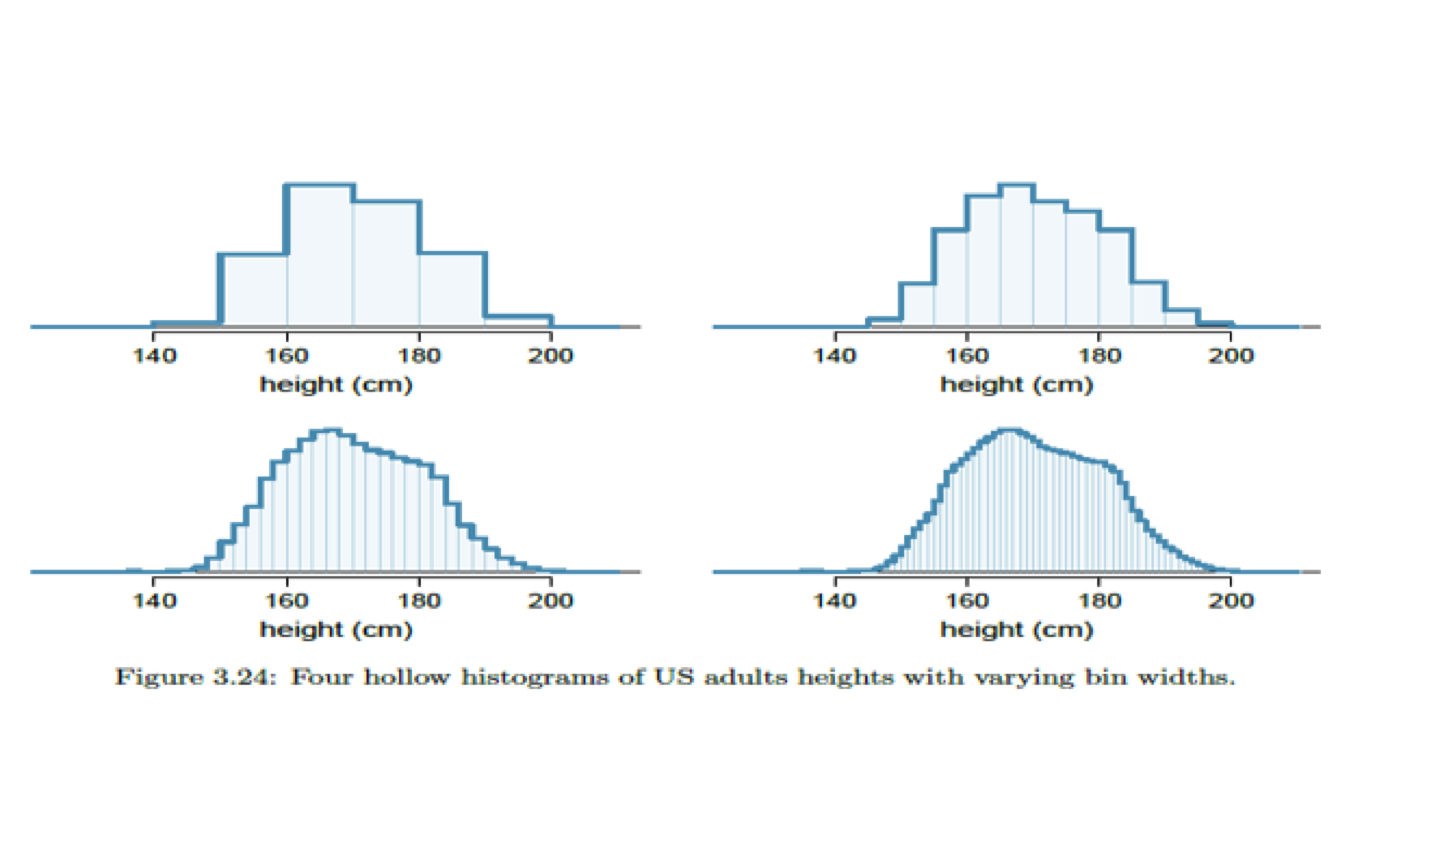
\includegraphics[width=0.75\linewidth]{Section7.5-ComparingMeanWithANOVA_files/figure-beamer/unnamed-chunk-4-1} \end{center}
\end{frame}

\begin{frame}{Constant variance}
\protect\hypertarget{constant-variance}{}
\alert{Does this condition appear to be satisfied?}

\begin{center}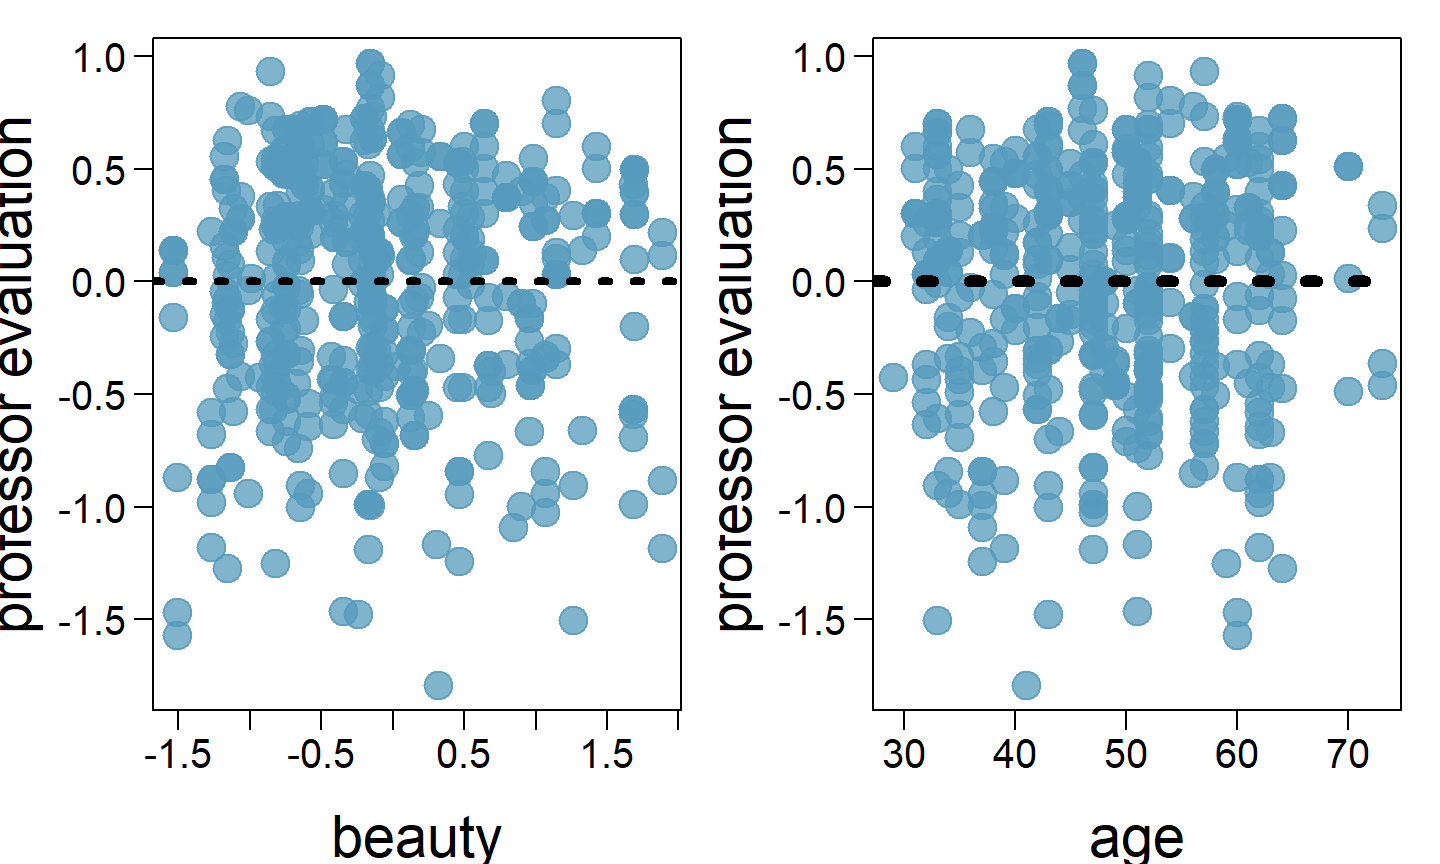
\includegraphics[width=0.75\linewidth]{Section7.5-ComparingMeanWithANOVA_files/figure-beamer/unnamed-chunk-5-1} \end{center}
\end{frame}

\begin{frame}{Which means differ?}
\protect\hypertarget{which-means-differ}{}
\begin{itemize}
\tightlist
\item
  Earlier we concluded that at least one pair of means differ. The
  natural question that follows is ``which ones?''
\end{itemize}

\pause

\begin{itemize}
\tightlist
\item
  We can do two sample \(t\) tests for differences in each possible pair
  of groups.
\end{itemize}

\pause

\alert{Can you see any pitfalls with this approach?}

\pause

\begin{itemize}
\item
  When we run too many tests, the Type 1 Error rate increases.
\item
  This issue is resolved by using a modified significance level.
\end{itemize}
\end{frame}

\begin{frame}{Multiple comparisons}
\protect\hypertarget{multiple-comparisons}{}
\begin{itemize}
\tightlist
\item
  The scenario of testing many pairs of groups is called
  \textbf{multiple comparisons}.
\end{itemize}

\pause

\begin{itemize}
\tightlist
\item
  The \textbf{Bonferroni correction} suggests that a more
  \alert{stringent} significance level is more appropriate for these
  tests:
\end{itemize}

\centering{$\alpha^* = \alpha / K$}

\raggedright where \(K\) is the number of comparisons being considered.

\pause

\begin{itemize}
\tightlist
\item
  If there are \(k\) groups, then usually all possible pairs are
  compared and \(K = \frac{k(k-1)}{2}\)
\end{itemize}
\end{frame}

\begin{frame}{Determining the modified \(\alpha\)}
\protect\hypertarget{determining-the-modified-alpha}{}
\alert{In the aldrin data set depth has 3 levels: bottom, mid-depth, and surface. If $\alpha = 0.05$, what should be the modified significance level for two sample $t$ tests for determining which pairs of groups have significantly different means?}

\begin{enumerate}
[A)]
\item
  \(\alpha^* = 0.05\)
\item
  \(\alpha^* = 0.05/2 = 0.025\)
\item
  \(\alpha^* = 0.05/3 = 0.0167\)
\item
  \(\alpha^* = 0.05/6 = 0.0083\)
\end{enumerate}
\end{frame}

\begin{frame}{Determining the modified \(\alpha\)}
\protect\hypertarget{determining-the-modified-alpha-1}{}
\alert{In the aldrin data set depth has 3 levels: bottom, mid-depth, and surface. If $\alpha = 0.05$, what should be the modified significance level for two sample $t$ tests for determining which pairs of groups have significantly different means?}

\begin{enumerate}
[A)]
\item
  \(\alpha^* = 0.05\)
\item
  \(\alpha^* = 0.05/2 = 0.025\)
\item
  \textcolor{red}{$\alpha^* = 0.05/3 = 0.0167$}
\item
  \(\alpha^* = 0.05/6 = 0.0083\)
\end{enumerate}
\end{frame}

\begin{frame}{Which means differ?}
\protect\hypertarget{which-means-differ-1}{}
\alert{Based on the box plots below, which means would you expect to be significantly different?}

\begin{columns}

\begin{column}{0.6\textwidth}


\begin{center}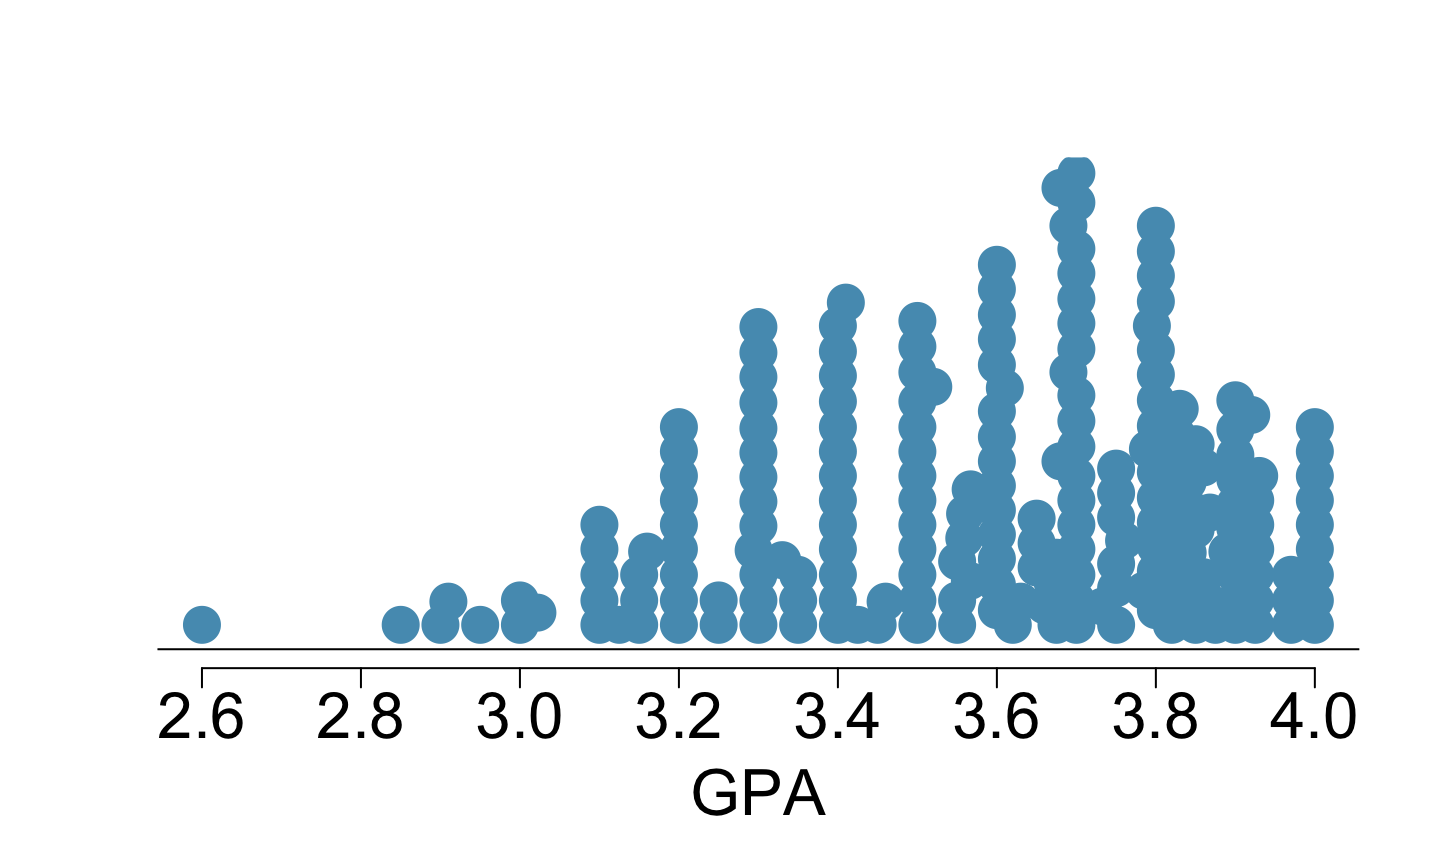
\includegraphics[width=1\linewidth]{Section7.5-ComparingMeanWithANOVA_files/figure-beamer/unnamed-chunk-6-1} \end{center}

\end{column}

\begin{column}{0.35\textwidth}

\small
A) bottom \& surface

B) bottom \& mid-depth

C) mid-depth \& surface

D) bottom \& mid-depth; \\ mid-depth \& surface

E) bottom \& mid-depth; \\ bottom \& surface; \\ mid-depth \& surface

\end{column}

\end{columns}
\end{frame}

\begin{frame}{Which means differ?}
\protect\hypertarget{which-means-differ-2}{}
If the ANOVA assumption of equal variability across groups is satisfied,
we can use the data from all groups to estimate variability:

\begin{itemize}
\item
  Estimate any within-group standard deviation with \(\sqrt{MSE}\),
  which is \(s_{pooled}\).
\item
  Use the error degrees of freedom, \(n-k\), for \(t\)-distributions.
\end{itemize}

\textbf{Difference in two means: after ANOVA}

\centering{$SE = \sqrt{\frac{\sigma_1^2}{n_1}+\frac{\sigma_2^2}{n_2}} \approx \sqrt{\frac{MSE}{n_1}+\frac{MSE}{n_2}}$}
\end{frame}

\begin{frame}{}
\protect\hypertarget{section-1}{}
\alert{Is there a difference between the average aldrin concentration at the bottom and at mid depth?}

\begin{columns}

\begin{column}{0.4\textwidth}
\scriptsize
\begin{center}
\begin{tabular}{l | c c c}
        & n & mean  & sd        \\
\hline
bottom  & 10    & \alert{6.04}  & 1.58 \\
middepth& 10    & \alert{5.05}  & 1.10 \\
surface & 10    & 4.2   & 0.66 \\
\hline
overall & 30    & 5.1       & 1.37
\end{tabular}
\end{center}
\end{column}

\begin{column}{0.7\textwidth}
\scriptsize
\begin{center}
\begin{tabular}{l rrrrr}
\hline
            & Df    & Sum Sq    & Mean Sq   & F value   & Pr($>$F) \\ 
\hline
depth       & 2     & 16.96     & 8.48      & 6.13  & 0.0063 \\ 
Residuals   & \alert{27}    & 37.33     & \alert{1.38}      &       &  \\ 
\hline
Total           & 29    & 54.29 \\
\end{tabular}
\end{center}
\end{column}

\end{columns}

\begin{eqnarray*}
T_{df_E} &=& \frac{(\bar{x}_{bottom} - \bar{x}_{middepth})}{\sqrt{ \frac{MSE}{n_{bottom}} + \frac{MSE}{n_{middepth}} }} \\ 
\pause
T_{27} &=& \frac{( 6.04 - 5.05 )}{\sqrt{ \frac{1.38}{10} + \frac{1.38}{10} }} = \frac{0.99}{0.53}  =1.87 \\
\pause
0.05 &<& p-value < 0.10 \qquad \text{{\footnotesize (two-sided)}} \\
\pause
\alpha^\star &=& 0.05 / 3 = 0.0167
\end{eqnarray*}

\pause

\small Fail to reject \(H_0\), data do not provide convincing evidence
of a difference between average aldrin concentrations at bottom and mid
depth.
\end{frame}

\begin{frame}{Pairwise comparisons}
\protect\hypertarget{pairwise-comparisons}{}
\alert{Is there a difference between the average aldrin concentration at the bottom and at surface?}

\pause

\begin{eqnarray*}
T_{df_E} &=& \frac{(\bar{x}_{bottom} - \bar{x}_{surface})}{\sqrt{ \frac{MSE}{n_{bottom}} + \frac{MSE}{n_{surface}} }} \\ 
\pause
T_{27} &=& \frac{( 6.04 - 4.2 )}{\sqrt{ \frac{1.38}{10} + \frac{1.38}{10} }} = \frac{1.84}{0.53}  =3.47 \\
\pause
p-value = 0.0018 \qquad \text{\footnotesize (two-sided)} \\
\pause
\alpha^\star &=& 0.05 / 3 = 0.0167
\end{eqnarray*} \pause \small Reject \(H_0\), the data provide
convincing evidence of a difference between the average aldrin
concentrations at bottom and surface.
\end{frame}

\end{document}
